\begin{figure}[tb]
\centering
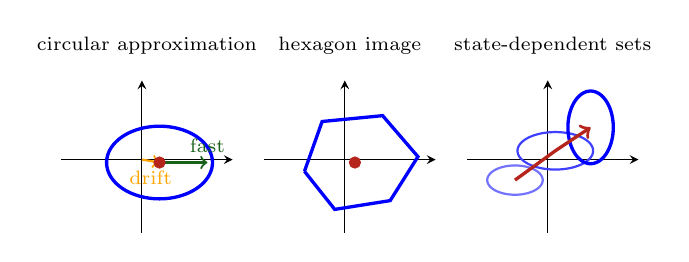
\begin{tikzpicture}[font=\scriptsize]
 \begin{axis}[name=a,width=.31\linewidth,height=.29\linewidth,axis lines=middle,
  xmin=-1.6,xmax=1.8,ymin=-1.25,ymax=1.35,ticks=none,title={circular approximation}]
  \addplot[blue,very thick,domain=0:360,samples=121] ({.35+1.05*cos(x)},{-.05+.62*sin(x)});
  \addplot[only marks,mark=*,BrickRed] coordinates {(.35,-.05)};
  \draw[->,Orange,thick] (axis cs:0,0)--(axis cs:.35,-.05) node[midway,below] {drift};
  \draw[->,ForestGreen!70!black,thick] (axis cs:.35,-.05)--(axis cs:1.3,-.05) node[above] {fast};
 \end{axis}
 \begin{axis}[name=b,at={(a.east)},anchor=west,xshift=4mm,width=.31\linewidth,height=.29\linewidth,
  axis lines=middle,xmin=-1.6,xmax=1.8,ymin=-1.25,ymax=1.35,ticks=none,title={hexagon image}]
  \addplot[blue,very thick] coordinates {(-.8,-.2)(-.2,-.85)(.9,-.7)(1.45,.05)(.75,.75)(-.45,.65)(-.8,-.2)};
  \addplot[only marks,mark=*,BrickRed] coordinates {(.2,-.05)};
 \end{axis}
 \begin{axis}[name=c,at={(b.east)},anchor=west,xshift=4mm,width=.31\linewidth,height=.29\linewidth,
  axis lines=middle,xmin=-1.6,xmax=1.8,ymin=-1.25,ymax=1.35,ticks=none,title={state-dependent sets}]
  \addplot[blue!55,thick,domain=0:360,samples=81] ({-0.65+.55*cos(x)},{-.35+.25*sin(x)});
  \addplot[blue!75,thick,domain=0:360,samples=81] ({.15+.75*cos(x+20)},{.15+.32*sin(x+20)});
  \addplot[blue,very thick,domain=0:360,samples=81] ({.85+.45*cos(x-25)},{.55+.62*sin(x-25)});
  \addplot[BrickRed,very thick,->] coordinates {(-.65,-.35)(.15,.15)(.85,.55)};
 \end{axis}
\end{tikzpicture}
\caption{Local current-velocity sets.  An ellipsoidal converter model gives a
translated ellipse, the exact inverter gives corners, and nonlinear flux or
changing speed moves and deforms the speedometer along a trajectory.}
\label{fig:velocity-sets}
\end{figure}

